% ============================================================
%  SCHOLA DOMESTICA — Magister Mathematica
%  Level 1 | Week 8 | Day 5
%  UNIT A FINAL REVIEW — Numbers, Addition & Subtraction 0–10
%  Covers all skills Weeks 1–8
% ============================================================
\documentclass[12pt, letterpaper]{article}

\usepackage[top=1in, bottom=1in, left=1in, right=1in]{geometry}
\usepackage{fontenc}
\usepackage{inputenc}
\usepackage{lmodern}
\usepackage{microtype}
\usepackage{amsmath}
\usepackage{graphicx}
\usepackage{xcolor}
\usepackage{tikz}
\usepackage{array}
\usepackage{enumitem}
\usepackage{multicol}
\usepackage{mdframed}
\usepackage{fancyhdr}

\definecolor{scholared}{RGB}{160,30,30}
\definecolor{scholagold}{RGB}{180,140,40}
\definecolor{scholacream}{RGB}{253,248,235}
\definecolor{scholagreen}{RGB}{50,110,60}
\definecolor{scholablue}{RGB}{40,80,140}

\pagestyle{fancy}
\fancyhf{}
\renewcommand{\headrulewidth}{0.6pt}
\fancyhead[L]{\small\textcolor{scholared}{\textbf{Schola Domestica — Magister Mathematica}}}
\fancyhead[R]{\small\textcolor{scholared}{Level 1 · Week 8 · Day 5 (Unit A Final)}}
\fancyfoot[C]{\small\textcolor{gray}{— \thepage\ —}}

\newcommand{\answerline}{\underline{\hspace{2.5cm}}}
\newcommand{\biganswerline}{\underline{\hspace{4cm}}}
\newcommand{\numbox}{\fbox{\hspace{0.6cm}\vphantom{0}}}
\newcommand{\symbox}{\fbox{\hspace{0.7cm}}}

\newmdenv[
  backgroundcolor=scholacream,
  linecolor=scholared,
  linewidth=1.5pt,
  roundcorner=6pt,
  innertopmargin=8pt,
  innerbottommargin=8pt,
  innerleftmargin=10pt,
  innerrightmargin=10pt
]{lessonbox}

\newmdenv[
  backgroundcolor=white,
  linecolor=scholagold,
  linewidth=2pt,
  roundcorner=6pt,
  innertopmargin=8pt,
  innerbottommargin=8pt,
  innerleftmargin=10pt,
  innerrightmargin=10pt
]{scorebox}

\begin{document}

\begin{center}
  {\LARGE\textbf{\textcolor{scholared}{Unit A Final Review}}}\\[4pt]
  {\Large\textcolor{scholagold}{\textit{Numbers, Addition, and Subtraction 0–10}}}\\[6pt]
  {\large\textcolor{scholablue}{Weeks 1 through 8}}\\[6pt]
  {\small Name: \biganswerline \hspace{1cm} Date: \answerline}\\[4pt]
  {\small\textit{Work carefully. You may use the number line at the bottom of the page.}}
\end{center}

\vspace{4pt}
\noindent\textcolor{scholared}{\rule{\linewidth}{1.5pt}}
\vspace{6pt}

% ===== SECTION 1: COUNTING =====
\noindent\textcolor{scholared}{\large\textbf{Section 1 — Counting \& Ordering}} \hfill \textit{(6 pts)}

\bigskip
\noindent\textbf{1.} Count: \;

\begin{tikzpicture}[baseline=-0.5ex]
  \foreach \i in {1,...,9}{\filldraw[scholablue](\i*0.4,0)circle(0.13cm);}
\end{tikzpicture}
\hfill \answerline

\noindent\textbf{2.} Write 0–10 in order: \;
\numbox , \numbox , \numbox , \numbox , \numbox , \numbox , \numbox , \numbox , \numbox , \numbox , \numbox

\noindent\textbf{3.} Least to greatest: 10 \; 6 \; 8 \; 7 \; 9 \hspace{0.5cm}
\numbox $<$ \numbox $<$ \numbox $<$ \numbox $<$ \numbox

\bigskip
\noindent\textcolor{scholared}{\rule{\linewidth}{0.4pt}}

% ===== SECTION 2: COMPARE =====
\noindent\textcolor{scholared}{\large\textbf{Section 2 — Compare}} \hfill \textit{(6 pts)}

\bigskip
\begin{multicols}{3}
\noindent\textbf{4.} $8$ \; \symbox \; $6$ \\[12pt]
\noindent\textbf{5.} $9$ \; \symbox \; $9$ \\
\columnbreak
\noindent\textbf{6.} $0$ \; \symbox \; $7$ \\[12pt]
\noindent\textbf{7.} $10$ \; \symbox \; $8$ \\
\columnbreak
\noindent\textbf{8.} Before 8: \answerline \\[12pt]
\noindent\textbf{9.} Between 7 and 9: \answerline
\end{multicols}

\bigskip
\noindent\textcolor{scholared}{\rule{\linewidth}{0.4pt}}

% ===== SECTION 3: ADDITION =====
\noindent\textcolor{scholared}{\large\textbf{Section 3 — Addition}} \hfill \textit{(8 pts)}

\bigskip
\begin{multicols}{4}
\noindent\textbf{10.} $4+3=$ \numbox \\[10pt]
\noindent\textbf{11.} $6+0=$ \numbox \\
\columnbreak
\noindent\textbf{12.} $5+5=$ \numbox \\[10pt]
\noindent\textbf{13.} $8+2=$ \numbox \\
\columnbreak
\noindent\textbf{14.} $2+7=$ \numbox \\[10pt]
\noindent\textbf{15.} $0+0=$ \numbox \\
\columnbreak
\noindent\textbf{16.} $3+6=$ \numbox \\[10pt]
\noindent\textbf{17.} $5+4=$ \numbox \\
\end{multicols}

\bigskip
\noindent\textcolor{scholared}{\rule{\linewidth}{0.4pt}}

% ===== SECTION 4: SUBTRACTION =====
\noindent\textcolor{scholared}{\large\textbf{Section 4 — Subtraction}} \hfill \textit{(8 pts)}

\bigskip
\begin{multicols}{4}
\noindent\textbf{18.} $7-3=$ \numbox \\[10pt]
\noindent\textbf{19.} $9-0=$ \numbox \\
\columnbreak
\noindent\textbf{20.} $10-4=$ \numbox \\[10pt]
\noindent\textbf{21.} $8-5=$ \numbox \\
\columnbreak
\noindent\textbf{22.} $6-2=$ \numbox \\[10pt]
\noindent\textbf{23.} $5-5=$ \numbox \\
\columnbreak
\noindent\textbf{24.} $9-3=$ \numbox \\[10pt]
\noindent\textbf{25.} $10-7=$ \numbox \\
\end{multicols}

\bigskip
\noindent\textcolor{scholared}{\rule{\linewidth}{0.4pt}}

% ===== SECTION 5: WORD PROBLEMS =====
\noindent\textcolor{scholared}{\large\textbf{Section 5 — Word Problems}} \hfill \textit{(4 pts)}

\bigskip
\noindent\textbf{26.} A nest has 6 eggs. 4 hatch. How many eggs remain unhatched?

\medskip
\hspace{2em} \numbox \; $-$ \; \numbox \; $=$ \; \numbox

\bigskip
\noindent\textbf{27.} There are 5 white doves and 3 grey doves. How many doves in all?

\medskip
\hspace{2em} \numbox \; $+$ \; \numbox \; $=$ \; \numbox

\bigskip
\noindent\textcolor{scholared}{\rule{\linewidth}{0.4pt}}

% ===== SECTION 6: ROMAN NUMERALS =====
\noindent\textcolor{scholared}{\large\textbf{Section 6 — Roman Numerals}} \hfill \textit{(4 pts)}

\bigskip
\noindent\textbf{28.} Write 7 in Roman numerals: \hfill \answerline \hspace{1cm}
\textbf{29.} What is IX? \hfill \answerline \\[8pt]
\noindent\textbf{30.} What is VIII? \hfill \answerline \hspace{1cm}
\textbf{31.} Write 10 in Roman numerals: \hfill \answerline

\bigskip
\noindent\textcolor{scholared}{\rule{\linewidth}{0.4pt}}

% NUMBER LINE (reference)
\begin{center}
\textit{Number Line — use if needed:}\\[6pt]
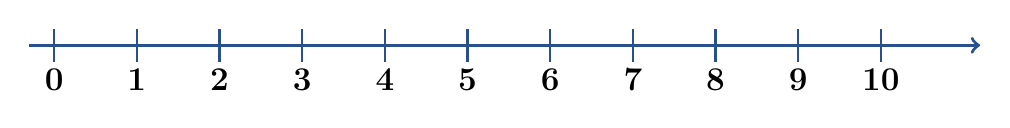
\begin{tikzpicture}[scale=1.05]
  \draw[very thick, scholablue, ->] (-0.3,0) -- (11.2,0);
  \foreach \n in {0,...,10} {
    \draw[thick, scholablue] (\n,0.2) -- (\n,-0.2);
    \node[below=5pt] at (\n,0) {\large\textbf{\n}};
  }
\end{tikzpicture}
\end{center}

\bigskip
\noindent\textcolor{scholared}{\rule{\linewidth}{1pt}}

% ===== SCORE =====
\begin{scorebox}
\begin{center}
\large\textbf{Score: \answerline / 36} \hspace{2cm}
\textbf{Parent/Teacher Initial: \answerline}\\[8pt]
\renewcommand{\arraystretch}{1.3}
\begin{tabular}{|l|l|}
\hline
33–36 & \textcolor{scholagreen}{\textbf{Excellent — ready for Unit B (Weeks 9–16)}} \\
\hline
27–32 & \textcolor{scholablue}{\textbf{Good — review weak sections, then proceed}} \\
\hline
Below 27 & \textcolor{scholared}{\textbf{Repeat relevant weeks before beginning Unit B}} \\
\hline
\end{tabular}
\end{center}
\end{scorebox}

\bigskip
\begin{lessonbox}
\textbf{Parent/Teacher Notes — What Comes Next:}\\[4pt]
\textbf{Unit B (Weeks 9–16)} introduces systematic addition and subtraction \textit{facts} for numbers 0–10.
Where Unit A built the \textit{concept}, Unit B builds \textit{fluency}.
Lessons become slightly longer (12–16 problems) and oral speed drills begin in Week 13.\\[4pt]
The child should be comfortable with: counting 0–10, writing numerals, comparing with $<\;>\;=$,
and the meaning of $+$ and $-$ before proceeding.
\end{lessonbox}

\end{document}
